%----------------------------------------------------------------
%	PACKAGES AND OTHER DOCUMENT CONFIGURATIONS
%----------------------------------------------------------------

\documentclass[landscape,a0paper,fontscale=0.285]{baposter} % Adjust the font scale/size here
\title{ETHz PAI Cheat Sheet}
\usepackage[brazilian]{babel}
\usepackage[utf8]{inputenc}

\usepackage{graphicx} % Required for including images
\graphicspath{{figures/}} % Directory in which figures are stored

\usepackage{xcolor}
\usepackage{colortbl}
\usepackage{tabu}

\usepackage{mathtools}
%\usepackage{amsmath} % For typesetting math
\usepackage{amssymb} % Adds new symbols to be used in math mode

\usepackage{booktabs} % Top and bottom rules for tables
\usepackage{enumitem} % Used to reduce itemize/enumerate spacing
\usepackage{palatino} % Use the Palatino font
\usepackage[font=small,labelfont=bf]{caption} % Required for specifying captions to tables and figures
\usepackage{bbding}

\usepackage{multicol} % Required for multiple columns
\setlength{\columnsep}{1.5em} % Slightly increase the space between columns
\setlength{\columnseprule}{0mm} % No horizontal rule between columns

\usepackage{tikz} % Required for flow chart
\usetikzlibrary{decorations.pathmorphing}
\usetikzlibrary{shapes,arrows} % Tikz libraries required for the flow chart in the template

\newcommand{\compresslist}{ % Define a command to reduce spacing within itemize/enumerate environments, this is used right after \begin{itemize} or \begin{enumerate}
\setlength{\itemsep}{1pt}
\setlength{\parskip}{0pt}
\setlength{\parsep}{0pt}
}

\definecolor{lightblue}{rgb}{0.145,0.6666,1} % Defines the color used for content box headers

\begin{document}

\begin{poster}
{
headerborder=closed, % Adds a border around the header of content boxes
colspacing=0.4em, % Column spacing
bgColorOne=white, % Background color for the gradient on the left side of the poster
bgColorTwo=white, % Background color for the gradient on the right side of the poster
borderColor=lightblue, % Border color
headerColorOne=lightblue, % Background color for the header in the content boxes (left side)
headerColorTwo=white, % Background color for the header in the content boxes (right side)
headerFontColor=white, % Text color for the header text in the content boxes
boxColorOne=white, % Background color of the content boxes
textborder=roundedleft, % Format of the border around content boxes, can be: none, bars, coils, triangles, rectangle, rounded, roundedsmall, roundedright or faded
eyecatcher=true, % Set to false for ignoring the left logo in the title and move the title left
headerheight=0.03\textheight, % Height of the header
headershape=roundedright, % Specify the rounded corner in the content box headers, can be: rectangle, small-rounded, roundedright, roundedleft or rounded
headerfont=\Large\bf\textsc, % Large, bold and sans serif font in the headers of content boxes
%textfont={\setlength{\parindent}{1.5em}}, % Uncomment for paragraph indentation
linewidth=1pt % Width of the border lines around content boxes
}
%----------------------------------------------------------------
%	TÍTULO
%----------------------------------------------------------------
{\bf\textsc{ETHz PAI Cheat Sheet}\vspace{0.0em}} % Poster title
{\textsc{ ETHz \ \ \ \ PAI \ \ \ \ \ C h e a t \ \ \ \ \ S h e e t \hspace{0pt}}}


%------------------------------------------------
% BÁSICO DO PYTHON
%------------------------------------------------
\headerbox{Probability \& BLR}{name=objectives,column=0,row=0}{

%--------------------------------------
\colorbox[HTML]{CCFFFF}{\makebox[\textwidth-2\fboxsep][l]{\bf - Gaussian}}

$P(\mathcal N | \mathcal N)\sim \mathcal N(\mu_{A|B},\Sigma_{A|B})$
\vspace{-0.3cm}
$$\vspace{-0.2cm}
\begin{aligned}
\mu_{A|B} &= \mu_A + \Sigma_{AB}\Sigma_{BB}^{-1}(x_B - \mu_B)
\\
\Sigma_{A|B} &= \Sigma_{AA} - \Sigma_{AB}\Sigma_{BB}^{-1}\Sigma_{BA}
\end{aligned}
$$


$P(M \mathcal N)\sim \mathcal N(\mu_Y, \Sigma_Y)$
\vspace{-0.3cm}
$$\vspace{-0.2cm}
\begin{aligned}
\mu_Y &= M\mu_X\\
\Sigma_{YY} &= M^\top\Sigma_{XX}M
\end{aligned}
$$

$P(\mathcal N + \mathcal N) \sim P(\mu_{Y}, \Sigma_Y)$
\vspace{-0.3cm}
$$\vspace{-0.2cm}
\begin{aligned}
\mu_{Y} &= \mu_X + \mu_{X'}\\
\Sigma_{YY} &= \Sigma_{X} + \Sigma_{X'}
\end{aligned}
$$

$P(\mathcal N \mathcal N) \sim P(\mu_{Y}, \Sigma_Y)$
\vspace{-0.3cm}
$$\vspace{-0.2cm}
\begin{aligned}
\Sigma_{YY}&= (\Sigma_{XX}^{-1}+\Sigma_{X'X'}^{-1})^{-1}
\\
\mu_{Y} &= \Sigma_{YY}\Sigma_{XX}^{-1}\mu_X + \Sigma_{YY}\Sigma_{X'X'}^{-1}\mu_{X'}
\end{aligned}
$$

entropy: $ln(\sigma\sqrt{2\pi e})$ (max in all distribution at $\mu,\Sigma$)

%--------------------------------------
\colorbox[HTML]{CCFFFF}{\makebox[\textwidth-2\fboxsep][l]{\bf - KL-Divergence:}} 
\vspace{-0.3cm}
$$
D_{KL}(p\Vert q) = \int  p(x)log\frac{p(x)}{q(x)}dx = H(p\vert q) - H(p)
$$
\begin{itemize}\compresslist
    \item $D_{KL}(p||q)$(backward) : mode averageing 
    \item $D_{KL}(q||p)$(forward) : mode seeking
    
    $p\sim\mathcal N(0,diag(\sigma_1^2,\sigma_2^2))\Rightarrow\sigma_q^2 = \frac{2}{\sigma_1^{-2}+\sigma_2^{-2}}$
    
    $D_{KL}(q||p)$ is well defined if $q$ is a subset of $p$
    \item $q\sim \mathcal N(\mathbb E(p),Var(p)) \Rightarrow H(p\vert q)=H(q)$
\end{itemize}


%--------------------------------------
\colorbox[HTML]{CCFFFF}{\makebox[\textwidth-2\fboxsep][l]{\bf - Bayesian Linear Regression:}}
\vspace{-0.3cm}
$$\vspace{-0.2cm}
y = w^\top x + \epsilon\quad 
\textcolor{orange}{\epsilon\sim \mathcal N(0,\sigma_n^2)}
~
\textcolor{green}{w\sim\mathcal N(0,\sigma_p^2)}
$$
$$\vspace{-0.2cm}
P(w|Y,X) \sim \mathcal N(\mu,\Sigma)
$$
$$\vspace{-0.2cm}
\mu = \frac{1}{\sigma_n^2}\Sigma X^\top Y \quad
\Sigma = \left(\frac{1}{\sigma_n^2}X^\top X + \frac{1}{\sigma_p^2}I\right)^{-1}
$$
uncertainty: \textcolor{orange}{aleartoric(rand)} + \textcolor{green}{epistemic(know)}

\underline{\textbf{Online}}
\vspace{-0.4cm}

    $$\vspace{-0.2cm}
    X_{new}^\top X_{new} = X^\top X + x_{t+1}x_{t+1}^\top
    $$
    $$\vspace{-0.2cm}
    X_{new}^\top Y_{new} = X^\top Y + y_{t+1} x_{t+1}
    $$


\underline{\textbf{Fast}} : $\mathcal O(d^3) \rightarrow \mathcal O(d^2)$
\vspace{-0.4cm}
    $$\vspace{-0.2cm}
    (A+xx^\top)^{-1} = A^{-1} - \frac{(A^{-1}x)(A^{-1}x)^\top}{1+x^\top A^{-1}x}
    $$
    $$\vspace{-0.2cm}
    (X_{new}^\top X_{new} + \sigma_n^2 I )^{-1} = (\underset{A}{\underbrace{X^\top X + \sigma_n^2}} + x_{t+1}x_{t+1}^\top)^{-1}
    $$

\underline{\textbf{Bayesian Logistic Regression}}
\vspace{-0.2cm}
\begin{itemize}\compresslist
    \item posterior is not gaussian
    \item posterior is not closed 
    \item posterior log-density  is convex
    \item $\sigma\uparrow \rightarrow$ standard logistic regression
    \item posterior cannot cover by $\mathcal N$ variational infer   
\end{itemize}
}


\headerbox{GP \& Kalman Filter}{name=introduction,column=1,row=0}{

\colorbox[HTML]{CCFFFF}{\makebox[\textwidth-2\fboxsep][l]{\bf - Gaussian Process}}\vspace{-0.3cm}
$$
\begin{aligned}
y &= f(x) + \epsilon \quad \epsilon\sim\mathcal N(0,\sigma_n^2)
\\
&P(f|X,Y)\sim GP(f;\mu',k')
\\
\mu'_{x^*} &= \mu_{x^*} + K_{x^*X}(K_{XX}+\sigma_n^2I)^{-1}Y
\\
k'_{x^*x^*} &= K_{x^*x^*} - K_{x^*X}^\top (K_{XX}+\sigma_n^2I)^{-1}K_{x^*X}
\end{aligned}
$$
$\mathcal O(n^3)$ for the inverse operation

prediction in closed form 

\underline{\textbf{Kernel}}

\textit{RBF}\vspace{-0.3cm}
$$
k(u,v) = \sigma_F^2  exp\left(-\frac{(u-v)^2}{2l^2}\right)
$$
$l$:  length scale control the distance of data

$\sigma_F$ : output scale  control  the magnitude
$$
\begin{aligned}
\underset{l\rightarrow 0}{lim}~k(u,v) &= \sigma_F^2\delta(u-v)\\
\underset{l\rightarrow 0}{lim}~k'(x,x) &= k(x,x) - k_{xX}(K_{XX}+\sigma_n^2 I)^{-1}k_{xX}^\top \\
&= \frac{\sigma_F^2\sigma_n^2}{\sigma_F^2 + \sigma_n^2}
\end{aligned}
$$
\begin{center}
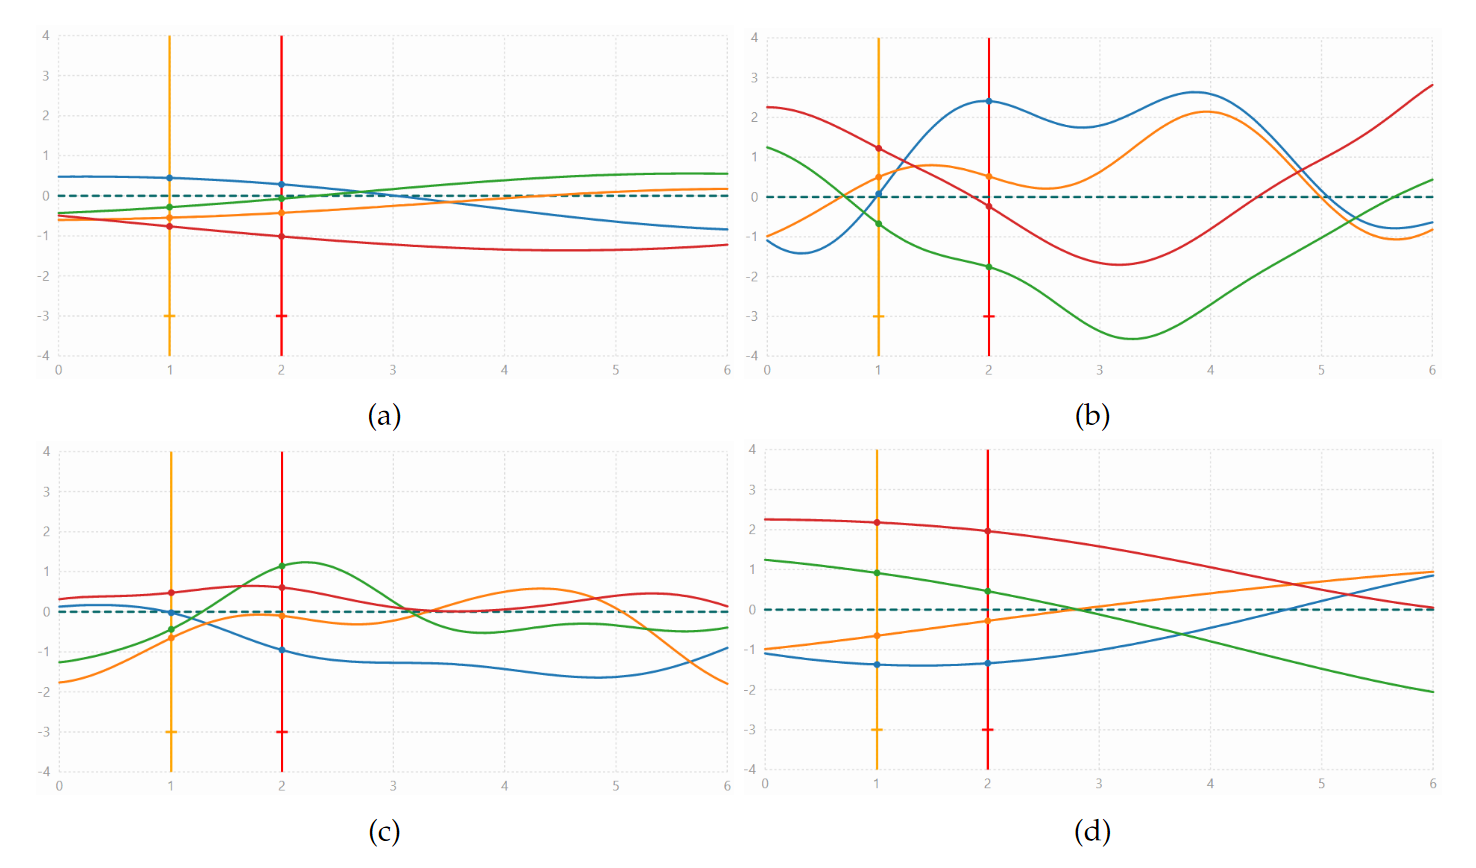
\includegraphics[width=0.9\textwidth, trim={0cm 3cm 0 2cm},clip]{figures/9ZdGX6UqMPl2WkR.png}
    \begin{tabular}{c | c}
         $\sigma_F^2=0.5\quad l=4$ & $\sigma_F^2=2\quad l=1$ \\\hline
         $\sigma_F^2=0.5\quad l=1$ & $\sigma_F^2=2\quad l=4$
    \end{tabular}
\end{center}

\textit{Linear}\vspace{-0.3cm}
$$
k(u,v) = \lambda uv
$$
equals to BLR with $\lambda  = \sigma_p^2$

\begin{center}
    

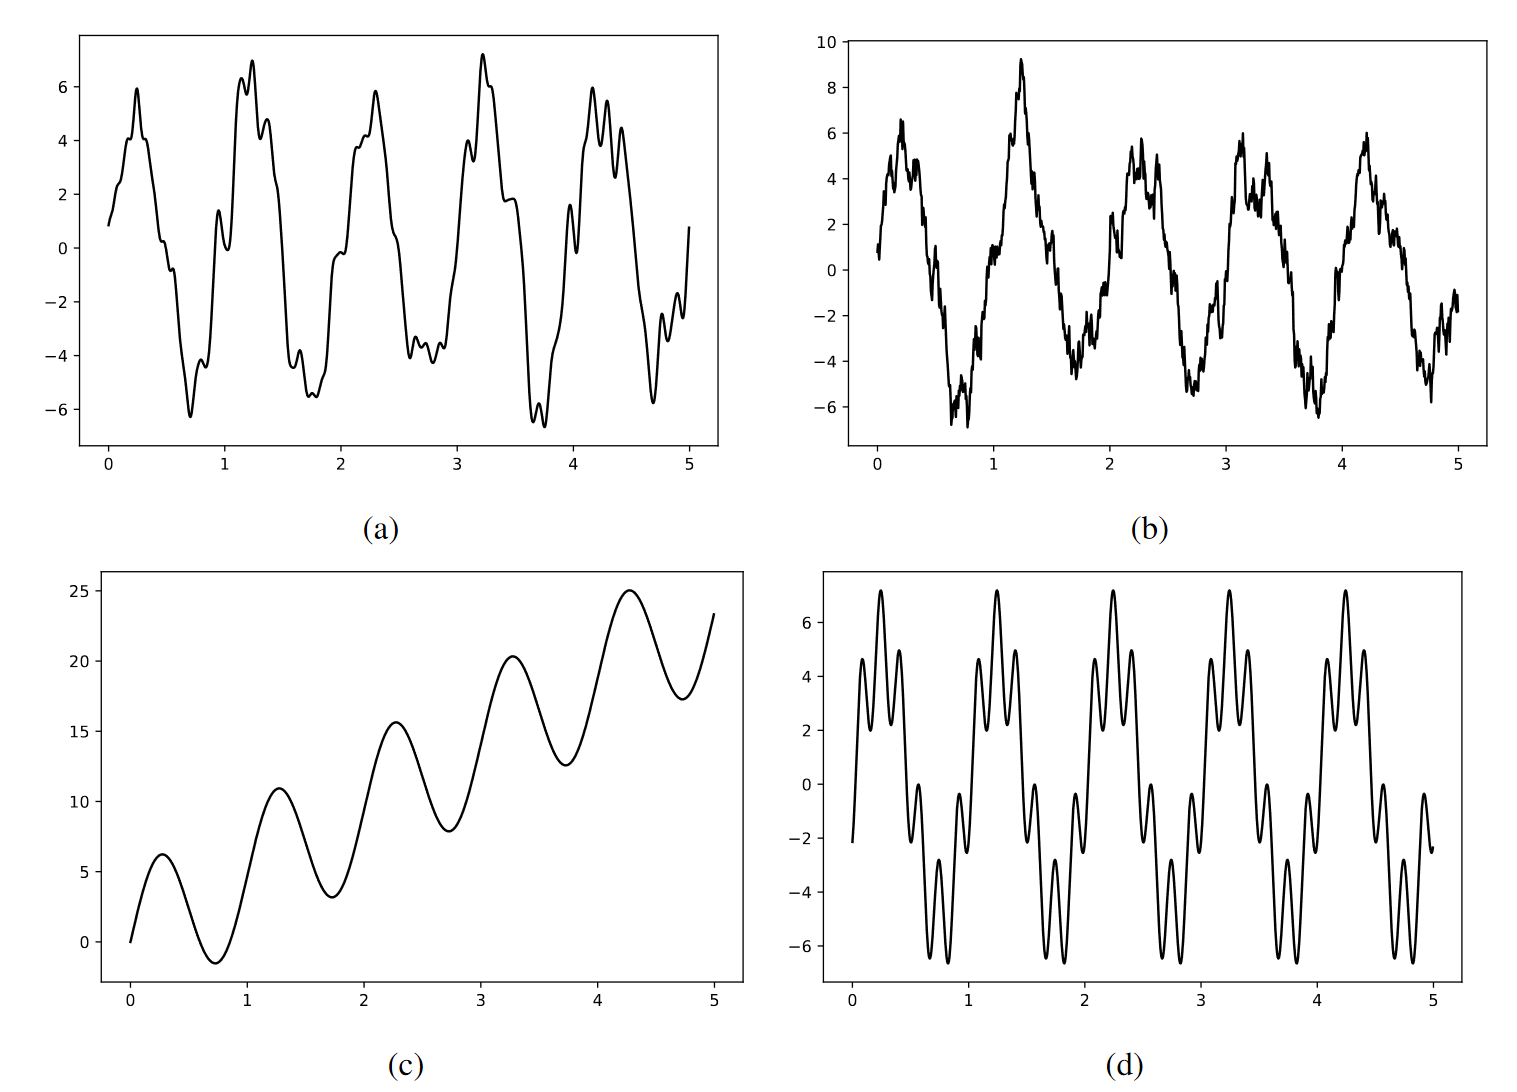
\includegraphics[width=0.9\textwidth,trim={0cm 3cm 0 2cm},clip]{figures/73sxNuLMZocVWTp.png}
    \begin{tabular}{c | c}
         $exp(-\lambda^2(x-y)^2)$ & $exp(-\lambda|x-y|)$ \\\hline
         $\lambda xy$ & $cos(2\lambda |x-y|)$
    \end{tabular}
\end{center}






}

\headerbox{GP \& Kalman Filter}{name=introduction,column=2,row=0}{

\underline{\textbf{Fast}}
\begin{itemize}\compresslist
    \item $k(x,x') = \phi(x)\phi(x)^\top~\mathcal O(n^3)\rightarrow \mathcal O(nm^2+m^3)$
    \item fourier features: $k(x,x') \approx k(x-x') $
    
    $=  \int_{\mathbb  R^d} p(\omega)e^{j\omega^top(x-x')}dw$ (stationary)
    
    Bochner Theorem:$p(\omega)\geq0 \Rightarrow k\geq 0$
    \item inducing points: $\mathcal O(n^3)$ 
    
        cubic inducing points, linear point
        
        SoR: subset of regressor (zero)
        
        FITC:  (diag)
\end{itemize}

\colorbox[HTML]{CCFFFF}{\makebox[\textwidth-2\fboxsep][l]{\bf - Kalman Filter}}\vspace{-0.3cm}
$$
x_{t+1} = F_tx_{t} + \Sigma_{x,t} \quad y_t  = H_t x_t + \Sigma_y
$$
$$
P(x_{t+1}|x_t) \sim \mathcal N(Fx_t, \Sigma_{x,t})
~
P(y_t | x_t) \sim \mathcal N(H_t x_t, \Sigma_y)
$$
\textbf{predict}\vspace{-0.4cm}
$$
\begin{aligned}
\hat x_{t+1} = F_t x_t \quad \hat \Sigma_{x,t+1} = H_t \Sigma_{x,t}H_t^\top + \Sigma_{d_t}
\end{aligned}
$$
$$
P(x_t|y_{1:t}) \sim \mathcal N(\mu_t, \Sigma_{d_t}^2)
$$
\textbf{correct}\vspace{-0.3cm}
$$
\begin{aligned}
K_{t+1} &= \hat \Sigma_{x,t}H_t^\top (H_t\hat \Sigma_{x,t}H_t^\top + \Sigma_y)^{-1}
\\
x_{t+1} &= \hat x_{t+1} + K_{t+1}(y_{t+1}-H_t\hat x_{t+1})\\
\Sigma_{x,t+1} &= (I-K_{t+1}H_t)\hat \Sigma_{x,t}
\end{aligned}
$$
kalman gain:$K_{t+1}$, can be computed offline

\underline{\textbf{Linear  Dynamic System}}
\vspace{-0.5cm}
$$
x_{k+1} \sim (a x_k,\sigma^2) , x_0=0 \rightarrow MLE(a) = \frac{\sum_{i=0}^{n-1}x_ix^{i+1}}{\sum_{i=0}^{n-1}x_i^2}
$$

if $a\sim \mathcal N(0, \frac{\sigma^2}{\lambda})$, $Var(a|x_0,\cdots,x_n) = \frac{\sigma^2}{\lambda + \sum_{i=0}^{n-1}x_i^2}$

\underline{\textbf{Wiener process/Brownian motion}}

assume $P(x_{t+1}|x_t)\sim\mathcal N(x_t,\sigma_x^2)\quad x_0\sim\mathcal N(0,\sigma_0^2)$, the Kalman Filter can be seen as a GP

$f\sim \mathcal{GP}(0, k_{KF})\quad k_{KF}(x,x') = \sigma_0^2 + \sigma_x^2 min\{x,x'\}$

\begin{center}
    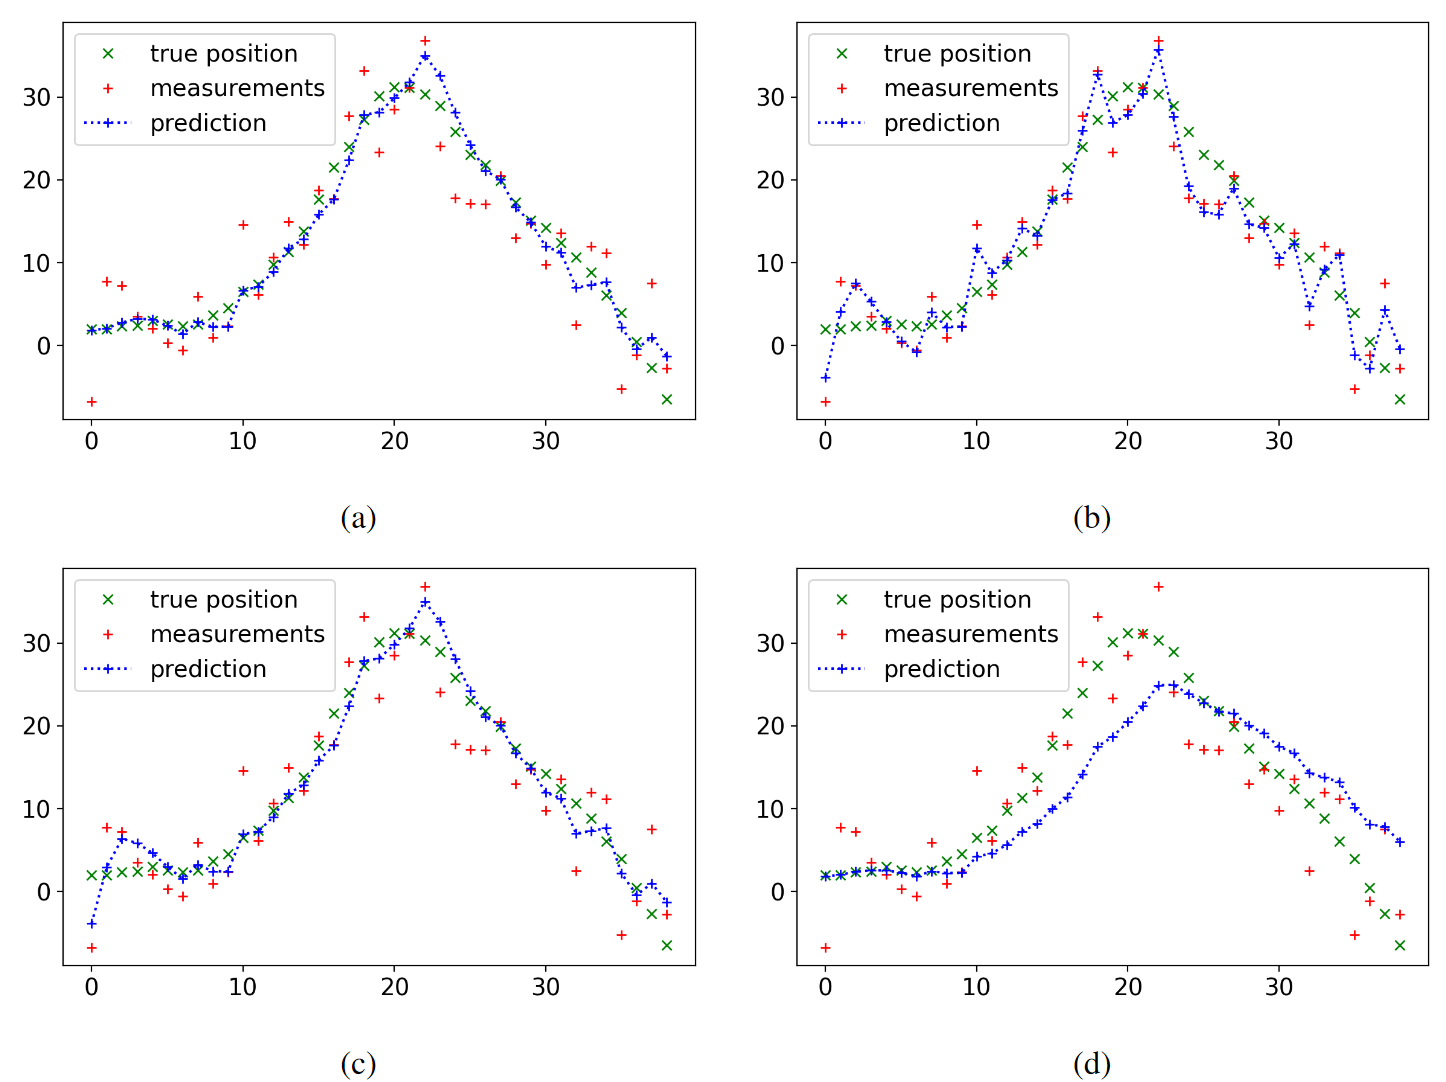
\includegraphics[width=0.8\textwidth,trim={0cm 4cm 0 3cm},clip]{figures/czu87jWDYg1FQRy.png}
\end{center}
\vspace{-0.3cm}
$$
\begin{aligned}
x_0\sim \mathcal N(\left[\begin{smallmatrix}
2,0
\end{smallmatrix}\right]^\top,\sigma^2 I) 
\\
x_{t+1} = 
\left[\begin{smallmatrix}
1 & 1 \\ 0 & a
\end{smallmatrix}\right]x_t
\quad
y_t\sim  \mathcal N (\left[\begin{smallmatrix}
    1 \\ 0 
\end{smallmatrix}\right] x_t, \sigma_y^2)
\end{aligned}
$$

\begin{tabular}{c|c}
    $a=1, \sigma=1, \sigma_y=1$& $a=1,\sigma=1,\sigma_y=1$ \\\hline
    $a=1, \sigma=10, \sigma_y=10$ & $a=0.5,\sigma=1,\sigma_y=10$ \\
\end{tabular}


}

%------------------------------------------------
% Approximation & Markov Chain Monte Carlo
%------------------------------------------------

\headerbox{Approximation \& MCMC}{name=results,column=3,span=1,row=0}{

\colorbox[HTML]{CCFFFF}{\makebox[\textwidth-2\fboxsep][l]{\bf - Approximation}}
\underline{\textbf{Laplacian approximation}}
\vspace{-0.3cm}
$$
q(\theta)\sim \mathcal (\hat\theta, \Lambda^{-1})~~
\hat\theta = \underset{\theta}{argmax}~p(\theta|y)~~
\Lambda = -\nabla\nabla p(\hat\theta|y)
$$
\vspace{-1.0cm}
\begin{itemize}\compresslist
    \item not skewed
    \item only one modal 
    \item no previous knowledge
\end{itemize}
\vspace{-0.5cm}
\begin{center}
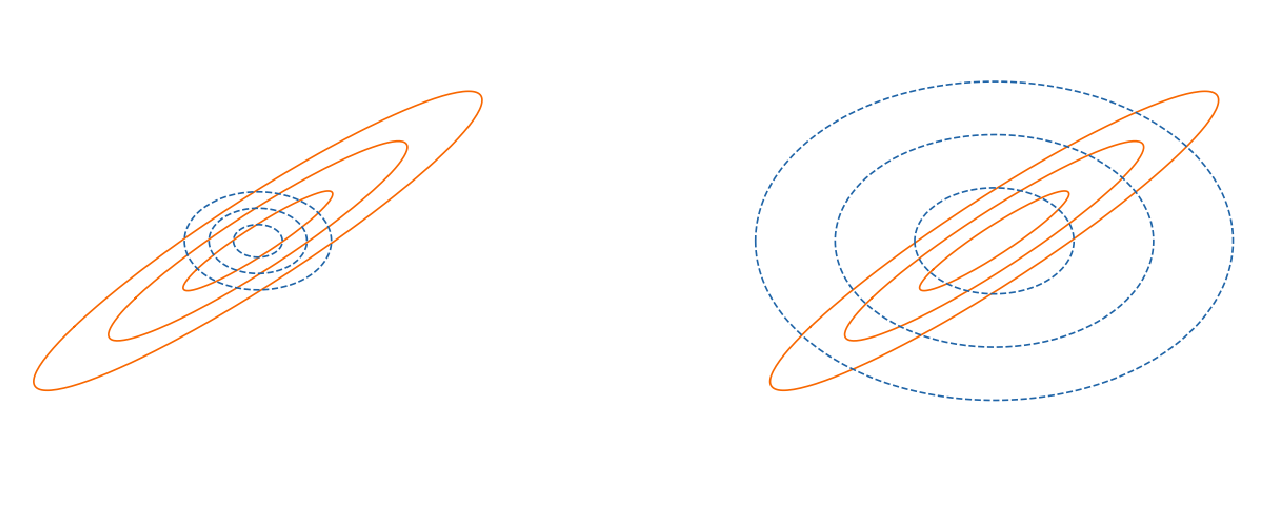
\includegraphics[width=0.8\textwidth, trim={0cm 3cm 0 2cm},clip]{figures/F5wAvc7PQ2CK3qB.png}
\end{center}
\vspace{-1cm}
\begin{itemize}\compresslist
    \item Left: backward KL $D_{KL}(\textcolor{lightblue}{q}\Vert \textcolor{orange}{p})$ 
    \item Right: forward KL $D_{KL}(\textcolor{orange}{p}\Vert \textcolor{lightblue}{q})$
\end{itemize}
\vspace{-0.3cm}
\underline{\textbf{Evidence Lower Bound(ELBO)}}
\vspace{-0.3cm}
$$\vspace{-0.2cm}
\begin{aligned}
Q^* &= \underset{Q\in\mathcal Q}{argmin}~D_{KL}(Q(Z)\Vert P(Z|X)) 
\\
&= \underset{Q\in\mathcal Q}{argmax}~\mathbb E_{Z\sim Q(Z)}[log(P(X|Z))] 
\\
&- D_{KL}(Q(Z)||P(Z)) = \mathbb E_q p - D_{KL}(p\Vert p)
\end{aligned}
$$

\textbf{MLE}
\vspace{-0.4cm}
$$\vspace{-0.2cm}
\hat \theta = \underset{\theta}{argmax}~P(X_{1:n}|\theta)
$$
sometimes add $l_2$ norm which is $\Vert \cdot - \mu \Vert_2^2$ for vector and $\Vert \cdot - \mu \Vert_F^2$ for matrix and $(\cdot-\mu)^2$ for scalar

\textbf{MAP}
\vspace{-0.3cm}
$$\vspace{-0.2cm}
\hat \theta = \underset{\theta}{argmax}(X_{1:n}|\theta,X')
$$
\textbf{reparameterization tricks}\vspace{-0.3cm}
\begin{itemize} \compresslist
    \item  random variable continous
    \item reduce variance by introducing bias
    \item automatic differentiation
\end{itemize}\vspace{-0.2cm}
\colorbox[HTML]{CCFFFF}{\makebox[\textwidth-2\fboxsep][l]{\bf - Markov Chain Monte Carlo}}
\vspace{-0.4cm}
$$\vspace{-0.3cm}
\pi = \pi P
$$

$\pi$ is the stationary state, $P$ is the transition matrix

\textbf{ergodic}:$\exists t\in \mathbb N \rightarrow (P)^t >0$
\vspace{-0.3cm}

\begin{itemize}\compresslist
    \item MCMC used for any distribution
    \item $P(x|x') = P(x'|x)\rightarrow$ uniform distribution
\end{itemize}
\vspace{-0.3cm}

\underline{\textbf{Metropolis-Hastings (MH) Algorithm}}:

given proposal transition $R(x'|x)$ and unnormalized stationary distribution $Q(x)$

accept rate $\alpha = min\{1, \frac{Q(x')R(x|x')}{Q(x)R(x'|x)}\}$ from $x$ to $x'$
% \vspace{0.1cm}

\underline{\textbf{Gibbs Sampling}} : random choose dimension

\underline{\textbf{MALA}}:
\vspace{-0.6cm}
$$\vspace{-0.3cm}
R(x'|x) = \mathcal N(x'|x-\tau \nabla f(x) ;2\tau I)
$$

\underline{\textbf{Stochastic Gradient Langevin Dynamics(SGLD)}}
\vspace{-0.4cm}
$$\vspace{-0.3cm}
\begin{aligned}
\Delta\theta &=  -\eta(\nabla log~p(\theta_t) + \frac{N}{n}\sum_{j=1}^n \nabla  log p(y_{i_{j}} | \theta_t, x_{i_j})) + \epsilon_t \\
& = -\eta(\theta_t + \nabla_\theta log~L(\theta_t)) + \epsilon_t\\
\epsilon_t &\sim \mathcal N(0, 2\eta I)\\
\end{aligned}
$$
$L(\theta_t)$ is the likelihood

can guarantee convergence, need burn in step




}






\end{poster}




\newpage



\begin{poster}
{
headerborder=closed, % Adds a border around the header of content boxes
colspacing=0.4em, % Column spacing
bgColorOne=white, % Background color for the gradient on the left side of the poster
bgColorTwo=white, % Background color for the gradient on the right side of the poster
borderColor=lightblue, % Border color
headerColorOne=lightblue, % Background color for the header in the content boxes (left side)
headerColorTwo=white, % Background color for the header in the content boxes (right side)
headerFontColor=white, % Text color for the header text in the content boxes
boxColorOne=white, % Background color of the content boxes
textborder=roundedleft, % Format of the border around content boxes, can be: none, bars, coils, triangles, rectangle, rounded, roundedsmall, roundedright or faded
eyecatcher=true, % Set to false for ignoring the left logo in the title and move the title left
headerheight=0.03\textheight, % Height of the header
headershape=roundedright, % Specify the rounded corner in the content box headers, can be: rectangle, small-rounded, roundedright, roundedleft or rounded
headerfont=\Large\bf\textsc, % Large, bold and sans serif font in the headers of content boxes
%textfont={\setlength{\parindent}{1.5em}}, % Uncomment for paragraph indentation
linewidth=1pt % Width of the border lines around content boxes
}
%----------------------------------------------------------------
%	TITLE SECTION 
%----------------------------------------------------------------

{\bf\textsc{E T H z \ \ \ \ P A I \ \ \ \ C h e a t \ \ \ \ S h e e t}\vspace{0.0em}} % Poster title
% {\textsc{ ETHz \ \ \ \ PAI \ \ \ \ \ C h e a t \ \ \ \ \ S h e e t \hspace{0pt}}}


%----------------------------------------------------------------
%	Outros Elementos
%----------------------------------------------------------------
\headerbox{Bayesian DL \& Optimization}{name=results,column=0,span=1,row=0}{
\colorbox[HTML]{CCFFFF}{\makebox[\textwidth-2\fboxsep][l]{\bf - Bayesian DeepLearning}}
\vspace{-0.1cm}
$$\vspace{-0.2cm}
P(y|x,\theta) \sim \mathcal N(y|f_\mu(x;\theta_\mu) , exp(f_\sigma(x;\theta_\sigma)))
$$
\textbf{train}
\vspace{-0.5cm}
$$\vspace{-0.2cm}
\begin{aligned}
\hat \theta &= \underset{\theta}{argmin} - lnP(\theta) - \sum_{i=1}^{n}lnP(y_i|x_i,\theta)
\\
&=  \underset{\theta}{argmin}~\lambda ||\theta||^2_2  +\frac{1}{2}\sum_{i=1}^n \left[\frac{||y_i-\mu(x_i;\theta_\mu)||^2}{\sigma(x_i;\theta_\sigma)^2} \right.\\ 
&\left. + ln~\sigma(x_i;\theta_\sigma)^2 \right]
\end{aligned}
$$

\textbf{predict}
\vspace{-0.6cm}
$$\vspace{-0.2cm}
P(y'|x',X,Y) = \mathbb E_{\theta\sim q}[P(y'|x',\theta)]
$$
$$\vspace{-0.3cm}
\begin{aligned}
Var[y'|x',X,Y] &= {\color{orange}\mathbb E_{\theta\sim q}[Var[y'|x',\theta]]}\\
&+{\color{green}Var[\mathbb E_{\theta\sim q}[y'|x',\theta]]}
\end{aligned}
$$
\begin{itemize}\compresslist
    \item \textcolor{orange}{Aleatoric uncertainty(random)} 
    \item \textcolor{green}{Epistemic uncertainty(knowledge)}
\end{itemize}
\vspace{-0.2cm}
\begin{itemize}\compresslist
    \item MAP for BNN is  not closed, unless likelihood and prior are $\mathcal N$
    \item MLE for BNN is closed
    \item $Var(C\theta|\theta) = 0 \quad \theta \sim p$
\end{itemize}
\vspace{-0.3cm}
approximate inference for BNN: 1.SGLD, 2.Dropout, 3.Ensemble, 4.black-box stochastic variational inference

% \vspace{-0.3cm}
\underline{\textbf{Stochastic Weight Averaging-Gaussian(SWAG)}}
\vspace{-0.3cm}
$$\vspace{-0.3cm}
\begin{aligned}
\mu_{SWA} &= \frac{1}{T}\sum_1^\top \theta_i\\
\Sigma_{SWA} &= \frac{1}{T-1}\sum_1^\top(\theta_i - \mu_{SWA})(\theta_i-\mu_{SWA})^\top
\end{aligned}
$$

\underline{\textbf{Dropout}}
\vspace{-0.3cm}
$$\vspace{-0.2cm}
p(y^*|x^*,X,Y) \approx \mathbb E_{\theta\sim q(\cdot|\lambda)}[p(y^*|x^*,\theta)]
$$
\begin{itemize}\compresslist
    \item dropout is also applied in prediction
    \item dropout can be seen as varational inference
\end{itemize}




\colorbox[HTML]{CCFFFF}{\makebox[\textwidth-2\fboxsep][l]{\bf - Bayesian Optimization}}
\underline{\textbf{Mutual Information}}
\vspace{-0.3cm}
$$\vspace{-0.3cm}
\begin{aligned}
F(s) &= H(f) - H(f|y_s) = \frac{1}{2}log|I+\sigma^{-2}K_s|
\\
F(S_T) &\ge (1-\frac{1}{e})\underset{S\subseteq D,|S|\le T}{max}~F(S)
\end{aligned}
$$

\underline{\textbf{regret}}
\vspace{-0.8cm}
$$\vspace{-0.4cm}
R_T = \sum_{t=1}^\top (max_{x\in D}f(x)-f(x_t))
$$
\begin{itemize}\compresslist
    \item sublinear(optimal) if $\frac{R_T}{T} \rightarrow 0$

    $\underset{t\rightarrow \infty}{lim}~f(x_t)\rightarrow f(x^*)$
    \item $R_T^A \le R_T^B$ cannot tell anything
    \item $\forall t~R_t^A \le R_t^B$ menas A is better
    \item $R\uparrow \rightarrow$ more exploration
\end{itemize}


}
\headerbox{Bayesian Optimization}{name=method,column=1}{

\colorbox[HTML]{CCFFFF}{\makebox[\textwidth-2\fboxsep][l]{\bf - Bayesian Optimization}}
\textbf{Uncertainty Sampling}
\vspace{-0.3cm}
$$\vspace{-0.3cm}
x_t = \underset{x\in D}{argmax} \frac{\textcolor{green}{\sigma_{e}^2(x)}}{\textcolor{orange}{\sigma_a(x)}}
$$
\vspace{-0.3cm}
\begin{itemize}\compresslist
    \item[\checkmark] max info gain in homoscedastic noise case
    \item[\XSolidBrush] max info gain in heterodastic noise 
    \item[\checkmark] $\underset{t\rightarrow \infty}{lim}~\hat x_t = \underset{x\in D}{argmax}~\mu_t(x)$, $f(\hat x )\rightarrow f(x^*)$
    \item[\XSolidBrush] $\underset{t\rightarrow \infty}{lim} f(x_t)\rightarrow f(x^*)$
\end{itemize}

\underline{\textbf{Upper Confidence Sampling(UCB)}}
\vspace{-0.3cm}
$$\vspace{-0.3cm}
a = \mu_t(x) + \beta \sigma_t(x)
$$
\vspace{-0.3cm}
\underline{\textbf{Probability of Improvement(PI)}}
$$\vspace{-0.3cm}
a = \Phi\left(\frac{\mu_t(x)-f^*}{\sigma_t(x)}\right)
$$
\vspace{-0.3cm}
\underline{\textbf{Expected Improvement(EI)}}
$$\vspace{-0.3cm}
\begin{aligned}
a &= (\mu_t(x)-f^*)\Phi\left(\frac{\mu_t(x)-f^*}{\sigma_t(x)}\right) \\
&+ \sigma_t(x)\phi\left(\frac{\mu_t(x)-f^*}{\sigma_t(x)}\right)
\end{aligned}
$$
\vspace{-0.3cm}
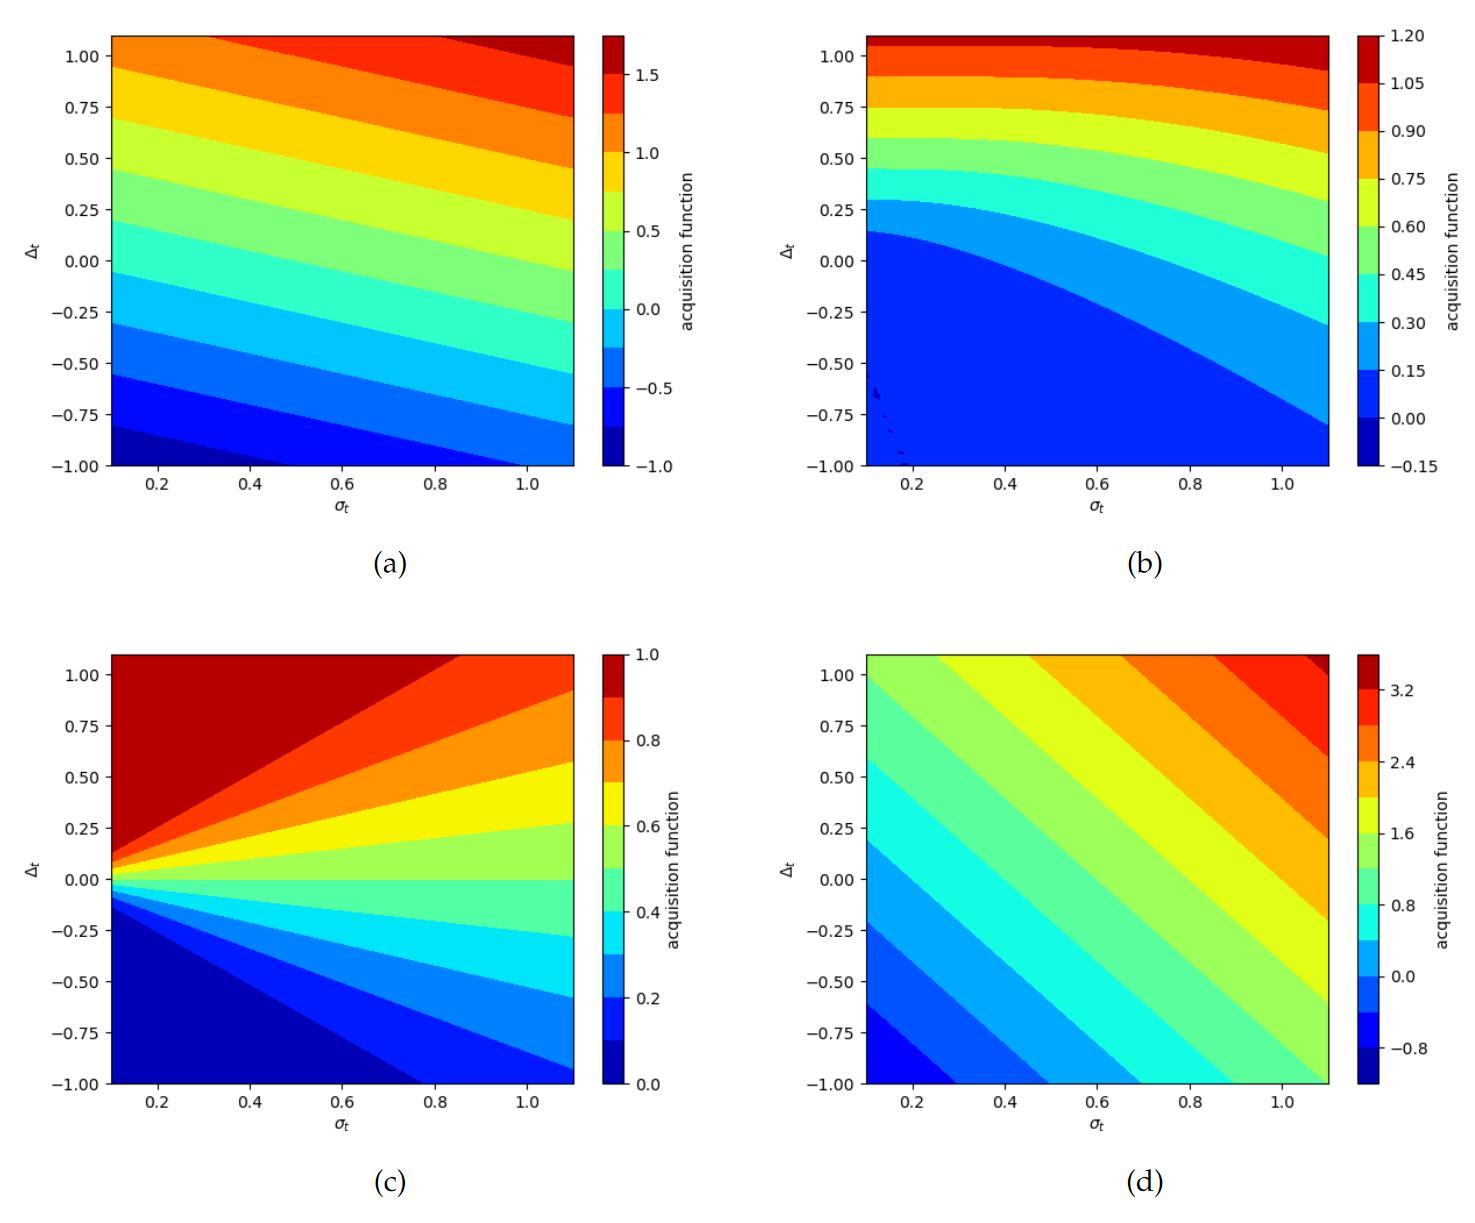
\includegraphics[width=0.9\textwidth, trim={0cm 1cm 0 0.2cm},clip]{figures/yzAfp5mekGTuO7w.png}
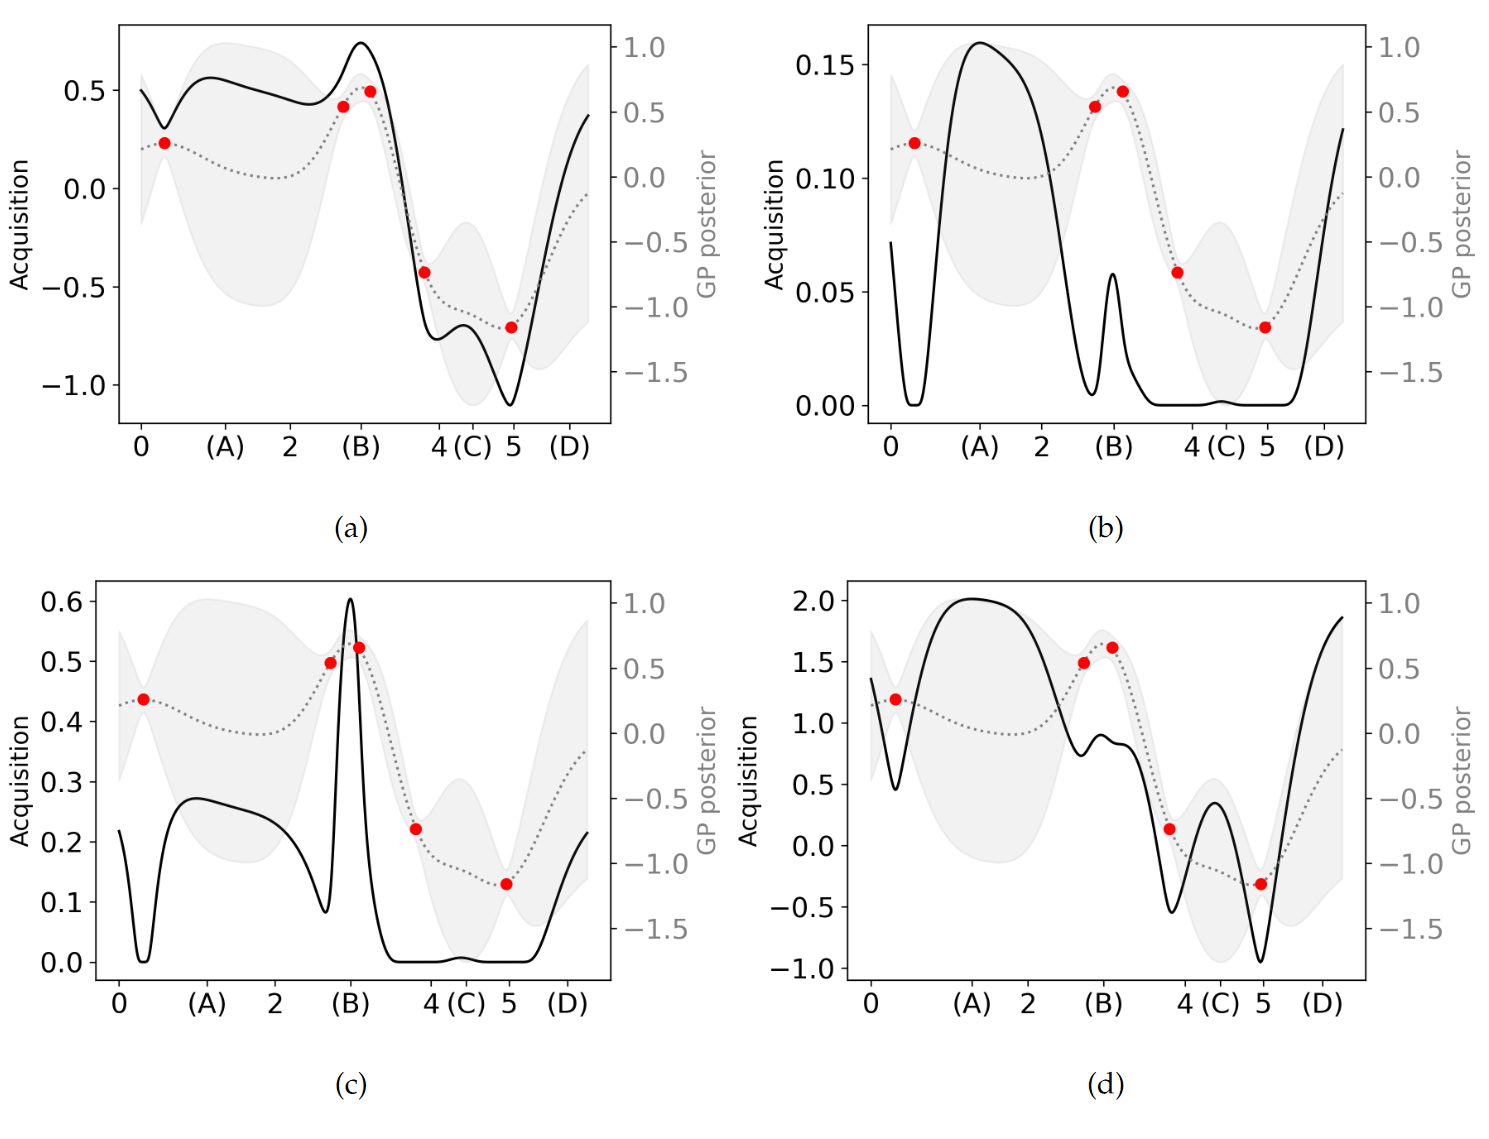
\includegraphics[width=0.8\textwidth,trim={0cm 1cm 0 0.2cm},clip]{figures/FqXAlIgS45KoYxp.png}
\centering{
\begin{tabular}{c|c}
     UCB($\beta=0.5$) & EI\\\hline
     PI & UCB($\beta=2$)
\end{tabular}
}

\vspace{-0.3cm}
$$\vspace{-0.4cm}
acquisition\uparrow \Longleftrightarrow exploitation
$$
\vspace{-0.3cm}
$$\vspace{-0.4cm}
acquisition\downarrow \Longleftrightarrow exploration
$$
\vspace{-0.3cm}


}

%----------------------------------------------------------------
%	Operadores
%----------------------------------------------------------------
\headerbox{Reinforcement Learning}{name=results2,column=2}{
\textbf{Bellman Theorem}
\vspace{-0.3cm}
$$
V^*(x) = max_a(r(x,a) + \gamma\sum_{x'}P(x'|x,a)V^*(x'))
$$
\textbf{Hoeffding Bound}
\vspace{-0.3cm}
$$
P(|\mu - \frac{1}{n}\sum_{i=1}^n Z_i|>\varepsilon) \leq 2exp(-\frac{2n\varepsilon^2}{C^2})
$$
\begin{itemize}
    \item $cR$ do not change policy
\end{itemize}
\colorbox[HTML]{CCFFFF}{\makebox[\textwidth-2\fboxsep][l]{\bf - Model Based}}

\underline{\textbf{Value Iteration}}\vspace{-0.3cm}
\begin{itemize}\compresslist
    \item guarantee converge to an \underline{$\varepsilon$ optimal policy} not the exact optimal policy
    \item polynomial time
    \item performance depend on the input
\end{itemize}
\underline{\textbf{Policy Iteration}}\vspace{-0.3cm}
\begin{itemize}\compresslist
    \item monotonically improve the policy
    \item polynomial time, gaurantee converge
\end{itemize}
\underline{\textbf{$\epsilon$ greedy}}

when random number $<\epsilon$ do the random action 

\underline{\textbf{Rmax method}}

set reward $R$ and transition probability $P(x^*|x,a)=1$ at first
\begin{itemize}\compresslist
    \item with probability $1-\sigma$,reach $\varepsilon$ - optimal
    \item polynomial time in $|X|, |A|, T,\frac{1}{\varepsilon},log(\frac{1}{\delta})$
\end{itemize}



\colorbox[HTML]{CCFFFF}{\makebox[\textwidth-2\fboxsep][l]{\bf - Model Free}}


\underline{\textbf{Temporal Difference(TD) - Learning}}
\vspace{-0.2cm}
$$
\hat V^\pi (x)\leftarrow (1-\alpha_t)\hat V^\pi (x) + \alpha_t(r+\gamma\hat V^\pi (x'))
$$
on-policy 

Theorem:$
\sum_t\alpha_t=\infty,\sum_t\alpha_t^2 < \infty \Rightarrow P(\hat V^\pi\rightarrow  V^\pi) = 1
$

\underline{\textbf{Q-Learning}}


off-policy\vspace{-0.2cm}
$$\vspace{-0.3cm}
\hat Q^* \leftarrow (1-\alpha_t)\hat Q^*(x,a) + \alpha_t(r+\gamma \underset{a'}{max}\hat Q^*(x',a'))
$$
init : $\hat Q^*(x,a) = \frac{R_{max}}{1-\gamma}\Pi_{t=1}^{T_{init}}(1-\alpha_t)^{-1}$

Theorem: $\sum_t\alpha_t=\infty,\sum_t\alpha_t^2 < \infty \Rightarrow P(\hat Q^*\rightarrow  Q^*) = 1$  
\begin{itemize}\compresslist
    \item with probability $1-\sigma$,  R~max~ will reach an $\varepsilon$ - optimal
    \item polynomial time in $|X|, |A|, T,\frac{1}{\varepsilon},log(\frac{1}{\delta})$
    \item decay learning rate guarantee convergence
\end{itemize}
}


%----------------------------------------------------------------
%	Reinforcement Learning 2
%----------------------------------------------------------------
\headerbox{Deep RL}{name=conclusion,column=3,span=1,row=0}{
\colorbox[HTML]{CCFFFF}{\makebox[\textwidth-2\fboxsep][l]{\bf - Model Free}}
\underline{\textbf{Policy Search}}

\underline{\textbf{REINFORCE}}\vspace{-0.3cm}
$$
\begin{aligned}
\nabla_{\theta} J(\theta) &= \mathbb E_{\tau\sim p_\theta(\tau)}[\sum_{t=0}^\top\gamma^t(\sum_{t'=t}^\top\gamma^{t'-t}r_{t'})\nabla_\theta ln\pi_\theta(a_t|x_t)]
\\
\theta  &\leftarrow \theta + \eta_t \nabla_\theta J(\theta)
\end{aligned}
$$

\underline{\textbf{Actor-Critic}}
\vspace{-0.3cm}
$$
\begin{aligned}
\nabla_{\theta_\pi} J(\theta_\pi) &= \mathbb E_{(x,a)\sim \pi_{\theta_\pi}} 
[Q_{\theta_Q}(x,a)\nabla_{\theta_\pi}ln\pi_{\theta_\pi}(a|x)]
\\
\theta_\pi &\leftarrow \theta_\pi + \eta_t \nabla_{\theta_\pi}J(\theta_\pi)
\\
\theta_Q &\leftarrow \theta_Q - \eta_t(Q_{\theta_Q}(x,a) - r \\
&- \gamma Q_{\theta_Q}(x',\pi_{\theta_\pi}(x')))\nabla_{\theta_Q}Q_{\theta_Q}(x,a)
\end{aligned}
$$
\begin{itemize}\compresslist
    \item use a baseline to reduce variance in the gradient estimates
\end{itemize}

\underline{\textbf{Proximal Policy Optimization(PPO)}}

$$
\begin{aligned}
L_{\theta_k}(\theta_k) &= \mathbb E_{\tau \sim \pi_k}\sum_{t=0}^\infty \left[\frac{\pi_\theta(a|x)}{\pi_{\theta_k}(a|x)}\left(r + \gamma Q^{\pi_{\theta_k}}(x',a)\right.\right.\\
&\left.\left.-Q^{\pi_{\theta_k}}(x,a)\right)\right]
\\
\theta_k &\leftarrow \theta_k - \eta_t \nabla_{\theta_k}L_{
\theta_k}(\theta_k)
\end{aligned}
$$

\underline{\textbf{Deep Deterministic Policy Gradients(DDPG)}}
\begin{itemize}\compresslist
    \item randomly add noise ensure sufficient  exploration
\end{itemize}


\begin{tabular}{|c|c|}
    \hline
     on-policy &  REINFORCE, Actor-Critic, PPO \\
     \hline
     off-policy&  DDPG, TD3, SAC\\
     \hline
\end{tabular}

\colorbox[HTML]{CCFFFF}{\makebox[\textwidth-2\fboxsep][l]{\bf - Model Based}}

reduce sample complexity

\underline{\textbf{Random Shooting Method}}

Monte Carlo Tree Search

\underline{\textbf{PETS}}


\colorbox[HTML]{CCFFFF}{\makebox[\textwidth-2\fboxsep][l]{\bf - Other}}
\textbf{Bernoulli distribution}\vspace{-0.3cm}
$$\vspace{-0.3cm}
\begin{aligned}
Bernoulli(x;p) &= p^x(1-p)^{1-x}\\
\mathbb  E[Bernoulli(x;p)] &= p\\
\mathbb Var[Bernoulli(x;p)] &= p(1-p)
\end{aligned}
$$

\textbf{Poisson distribution}\vspace{-0.3cm}
$$
\begin{aligned}
Pr(x;\lambda) &= \frac{\lambda^k e^{-\lambda}}{k!}\\
\mathbb E[Pr(x;\lambda)] &= \lambda\\
\mathbb Var[Pr(x;\lambda)] &= \lambda\\
\end{aligned}
$$
%-----------------------------------
}
%----------------------------------------------------------------
%	REFERENCES  {name=objectives,column=0,row=0}
%----------------------------------------------------------------
%\headerbox{bb}{name=references,column=1,row=0}{}
%----------------------------------------------------------------
%	FUTURE RESEARCH
%----------------------------------------------------------------
%\headerbox{aa}{name=futureresearch,column=1,row=0}{}
%----------------------------------------------------------------
%	CONTACT INFORMATION
%----------------------------------------------------------------
%\headerbox{Contact Information}{name=contact,column=2,span=2,row=0}{}
%----------------------------------------------------------------
\end{poster}
\end{document}